\chapter{Resultados}
En este capitulo se presentan los resultados experimentales de el esquema presentado, para un experimento que se considera es representativo de los demás.


\section{Entorno Experimental}



\subsection{robot}
La plataforma que estamos usando es un robot cartesiano de 3 DOF visto en  \cref{fig:dsc9825}, se utiliza un generador de señal para el voltaje de entrada a los motores de corriente continua, estamos utilizando MATLAB como la interfaz entre el sistema de visión, el control y el generador de funciones.
\begin{figure}
	\centering
	\includegraphics[width=0.5\linewidth]{visio/visio3/coordenadasrobcam2}
	\caption{Representación de un Robot Cartesiano}
	\label{fig:coordenadasrobcam}
\end{figure}



\begin{figure}
	\centering
	\includegraphics[width=0.5\linewidth]{Imagenes/DSC_9825}
	\caption{}
	\label{fig:dsc9825}
\end{figure}

\clearpage

\subsection{\textit{Gripper}}
El \textit{Gripper} que vamos a utilizar es el modelo SCHUNK WSG-50 que aparece en \cref{fig:dsc9821}, tiene un observador de fuerza, utiliza una fuente de 24V, la abertura es de 10 cm y se puede utilizar con MATLAB para ser operado. \\
Para ser usado se necesitó establecer la comunicación con \textbf{MATLAB}, esta es comunicación básica, en la que se manda un paquete de datos que contiene el comando y las opciones, en el apéndice \ref{codewsg50}, aparece el código que se uso.

\begin{figure}
	\centering
	\includegraphics[width=0.7\linewidth]{Imagenes/DSC_9821}
	\caption{\textit{Gripper} modelo SCHUNK WSG-50}
	\label{fig:dsc9821}
\end{figure}


Se diseño la base para el \textit{Gripper}, y los dedos, se intenta usar el sensor de fuerza y momento, por lo que uno de los 2 dedos tiene una cavidad para este. en el apéndice \ref{label}, se puede encontrar el diseño que se uso.

en la imagen \ref{label}, se encuentra el resultado 


\clearpage

\subsection{cámara}

El sistema de visión usa una cámara RGBD que se muestra en la figura \ref{fig:dsc9822}, se uso un programa entre MATLAB y \textit{Openni} \cite{matlabwrapper}.

La cámara que se uso es el ASUS XTION PRO, su sensor de profundidad tiene un rango operativo de 0,8 metros a 3,5 metros, la resolución de la imagen de color y la imagen de profundidad es $480 \times640$, y la velocidad de fotogramas es 20 cuadros por segundo, ya que es la velocidad de fotogramas del sensor de profundidad. \\




\begin{figure}
	\centering
	\includegraphics[width=0.7\linewidth]{Imagenes/DSC_9823}
	\caption{Camara Asus Xtion live pro}
	\label{fig:dsc9823}
\end{figure}
\begin{figure}
	\centering
	\includegraphics[width=0.7\linewidth]{Imagenes/DSC_9824}
	\caption{}
	\label{fig:dsc9824}
\end{figure}

\clearpage
%\section{Protocolo de Experimentación}
%cual es el protocolo? como se disenaron los experimentos?




\section{Resultados Experimentales}

Los experimentos se diseñaronpara ser lo mas simples posbibles, por lo que solo se intetara buscar como es la respuesta alproblema specifico, sin agregar mas varibles, las cueles es seguro que existan en un ambiente real.
El experimento consiste en colocar un objeto del cual no se ha dado niguna informacion previa, en una zona conocida, que es el area de trabajo del robot, esta area es observada por una camara RGBd la cual tiene una vista frontal superior del area, aunque el unico requerimiento de la posicion de la camara es que la vista sea superior, se esta usando la vista frontal para facilitar la calibracion, pero el uso de una vista lateral es posible, minetras se tenga buena visivilidad del area, la vista superior tampoco es nesesario que sea mucho mayor, en los experimentos se esta usando una inclinacion hacia abajo de 15° a 30°. El\textit{Gripper}, esta conectado a la computadora central y estara pprocesando los datos de los sensores delrobot y el sensor de fuerza y momentos mecanicos que fue instalado en el \textit{Gripper}, la finalidad del experimento es encontrar el objeto y sujetarlo para moverlo a un area determinada.

A continuación se presentan los resultados de un experimento que se llevo acavo usando una pelota de plastico.;

En  \cref{fig:imagen1} se muestra la imagen de entrada, esta imagen en 3 dimensiones contiene las coordenadas X,Y,Z del escenario percibido, las unidades son milímetros.

\begin{figure}
	\centering
	
\includegraphics[width=1.2 \linewidth]{visio/graficasderesultados/imagen1}
	\caption{Imagen de profundidad}
	\label{fig:imagen1}
\end{figure}
\cref{fig:dsobel1}, es el resultado del primer algoritmo de visión, y este nos entrega los bordes de la imagen los cuales serán usados después para encontrar las coordenadas del centroide de cada objeto en el espacio. 
\begin{figure}
	\centering
	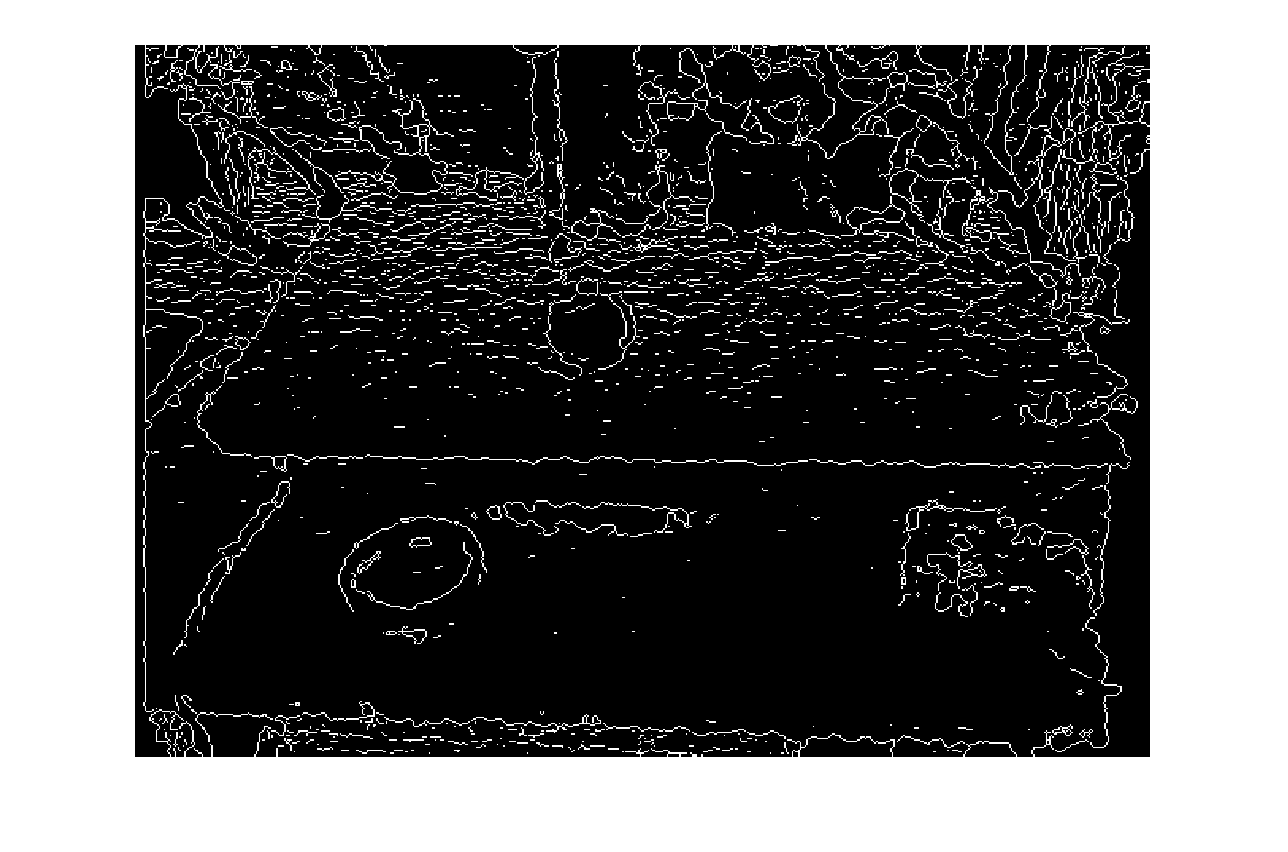
\includegraphics[width=.9\linewidth]{visio/graficasderesultados/Dsobel1}
	\caption{Bordes de la escena}.
	\label{fig:dsobel1}
\end{figure}

En la imagen \cref{fig:dbordes1},se puede observar la diferencia de las imágenes \cref{fig:imagen1} y \cref{fig:dsobel1}, la cual nos da una idea de cada objeto en la imagen, esta es solo representativa, ya que aunque podría ser útil para segmentar algún objeto, no se usa ya que habría problemas si l objeto es demasiado grande o las vistas son confusas, esto es que la distancia cambie mucho en n pequeño punto del objeto, lo que llevaría a segmentarlo como objetos distintos, por eso es necesario combinarlo con otro algoritmo para la segmentación.
\begin{figure}
	\centering
	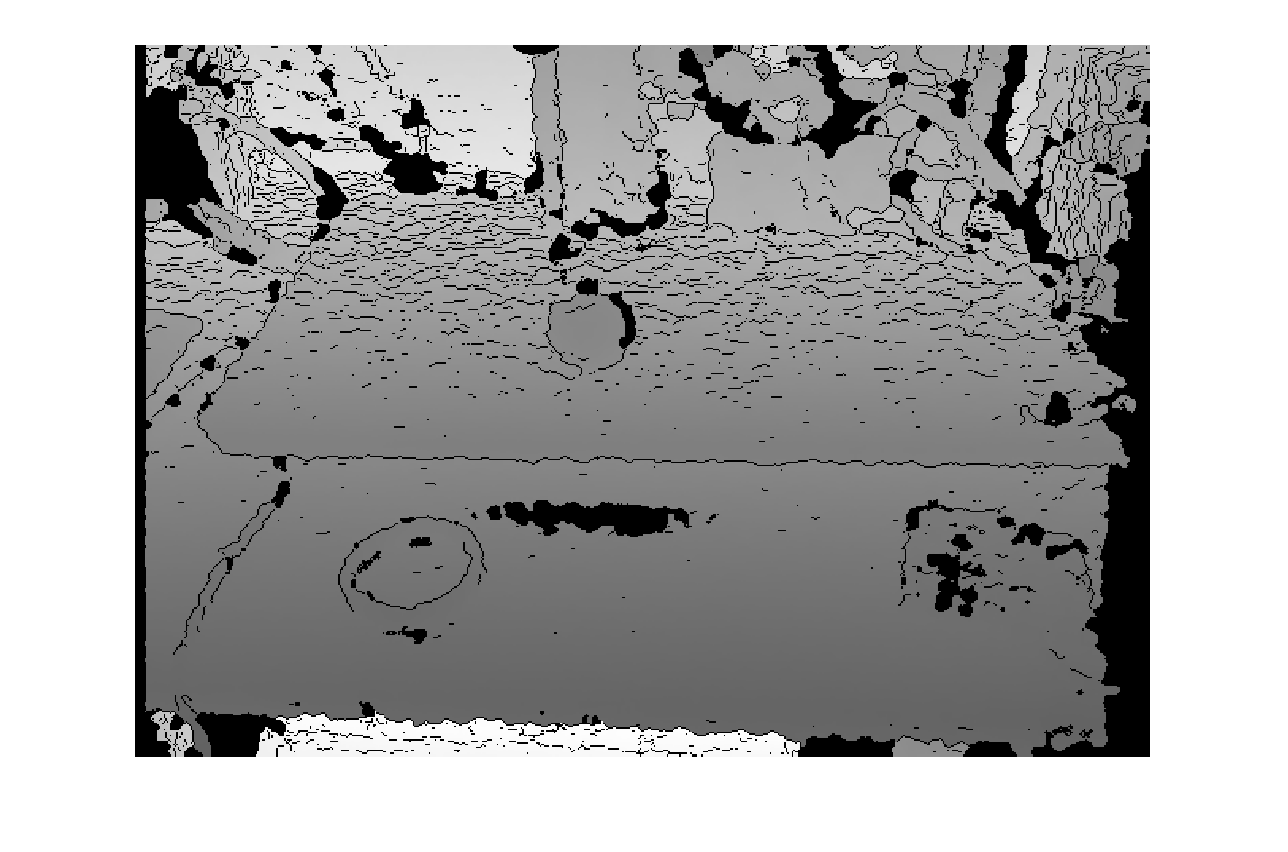
\includegraphics[width=.9\linewidth]{visio/graficasderesultados/Dbordes1}
	\caption{Imane ilustrativa del escenario si segmentara todo.}
	\label{fig:dbordes1}
\end{figure}



En \cref{temp1}, s puede apreciar el objeto segmentado, esto es porque en este ejemplo solo existía este objeto dentro del área de trabajo del  robot, por lo que se segmento fácilmente, \cref{dix1,diy1,diz1}, son los bodes de la imagen en sus respectivas dimensiones (X,Y,Z).

\begin{figure*}[h]
	\centering
	\begin{tabular}{cccc}
		%\hline 
		\subfloat[Objeto Segmentado]{		\includegraphics[width=.55\linewidth]{visio/graficasderesultados/temp1}\hspace{-1cm}\label{temp1}}
		
		\subfloat[sobel en x]{%
			\includegraphics[width=.55\linewidth]{visio/graficasderesultados/dix1}\hspace{-1cm}\label{dix1}}
		\\
		\subfloat[sobel en y]{%
			\includegraphics[width=.55\linewidth]{visio/graficasderesultados/diy1}\hspace{-1cm}\label{diz1}}
				\subfloat[sobel en y]{%
			\includegraphics[width=.55\linewidth]{visio/graficasderesultados/diz1}\hspace{-1cm}\label{diy1}}
		%	\hline 
	\end{tabular}
	\caption{resultados de los algoritmos 1 y 2}
	\label{fig2} 
\end{figure*}


Se puede observar en \cref{fig:erz1}, una linea, esta imagen se consiguió con el segundo algoritmo y es la que nos dará las coordenadas para posicionar el \textit{Gripper}. la linea representa el lugar en el que se encontrara el \textit{Gripper}, y los valores que estén sobre esa linea serán las coordenadas de (X,Y,Z). 
\begin{figure}
	\centering
	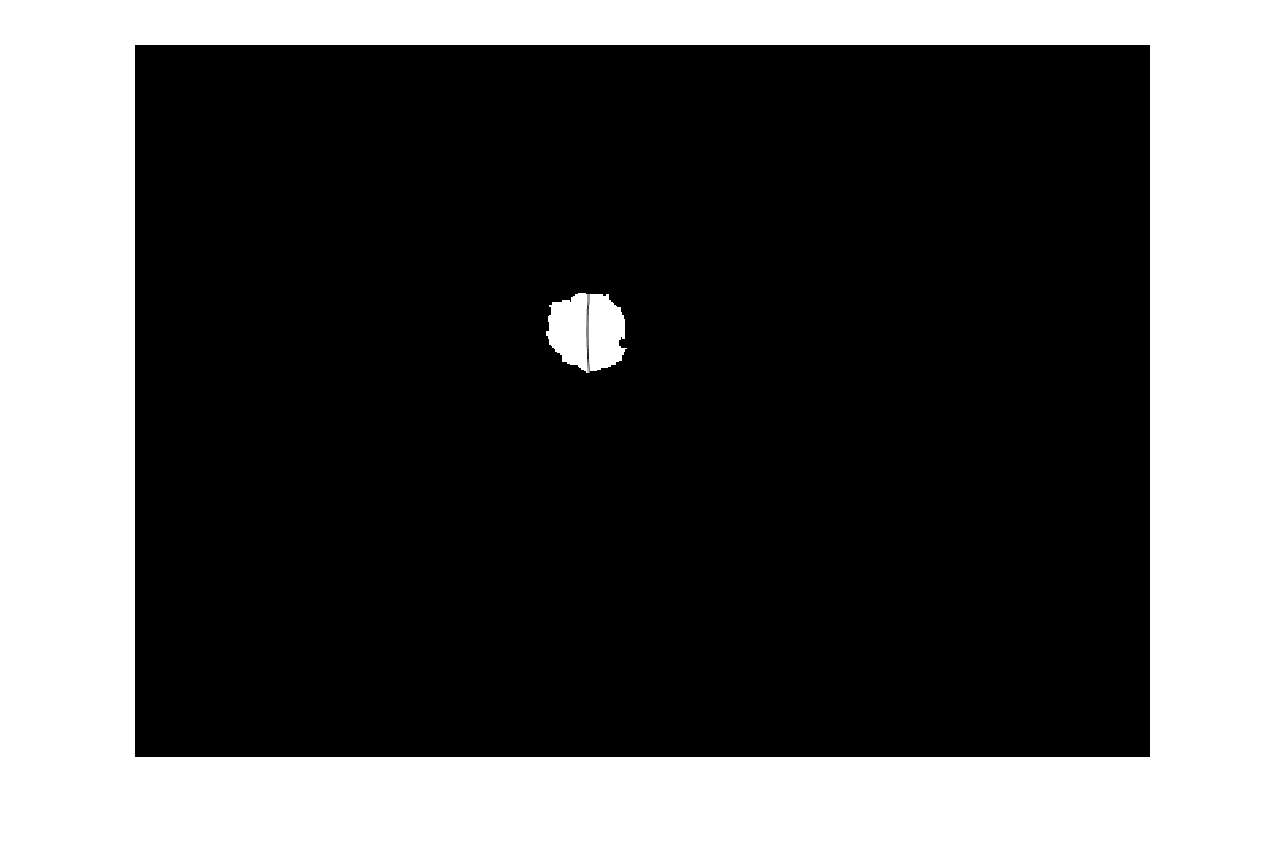
\includegraphics[width=1\linewidth]{visio/graficasderesultados/erz1}
	\caption{}
	\label{fig:erz1}
\end{figure}


\clearpage

Los resultados del control se pueden ver a continuación:
En \cref{fig:betasx1,fig:betasy1,fig:betasz1}, se encuentran los resultados de las constantes de aprendizaje $(\beta)$ de cada uno de los ejes del robot, a pesar de haber crecido a lo largo del experimento continúan creciendo cada vez que el eje correspondiente es movido, este es un problema ya que seguirá creciendo hasta que exista un sobrepaso en la respuesta, y es hasta ese momento en que comenzara a decrecer, manteniendo las ganancias en ese vecindario de valores, a pesar de eso se puede notar que la señal en \cref{fig:posicion1}, que la respuesta del control se mantiene trabajando de manera estable.
En \cref{fig:control1}, se observan las señales de control que se envían a cada eje, aquí se puede ver como la principal razón por la que no existe un sobrepaso, es porque las ganancias son muy  diferentes en cada punto de los valores de pertenencia, por lo que, aun con lo grande que son las ganancias de los extremos, estas caerán rápidamente a las ganancias cercanas a errores de cero, debido a que se reduce el error, por lo que no representan un problema a la hora de acercare demasiado a una posición deseada.
Pero eso no significa que no exista ese riesgo, ya que en algún momento debería llegarse a esa situación , a menos que se desactive el aprendizaje, o se cambie de ley de aprendizaje, pero aun si no se hace algo así, tardaría varios ciclos el que para que curra algo así.

\begin{figure}
	\centering
	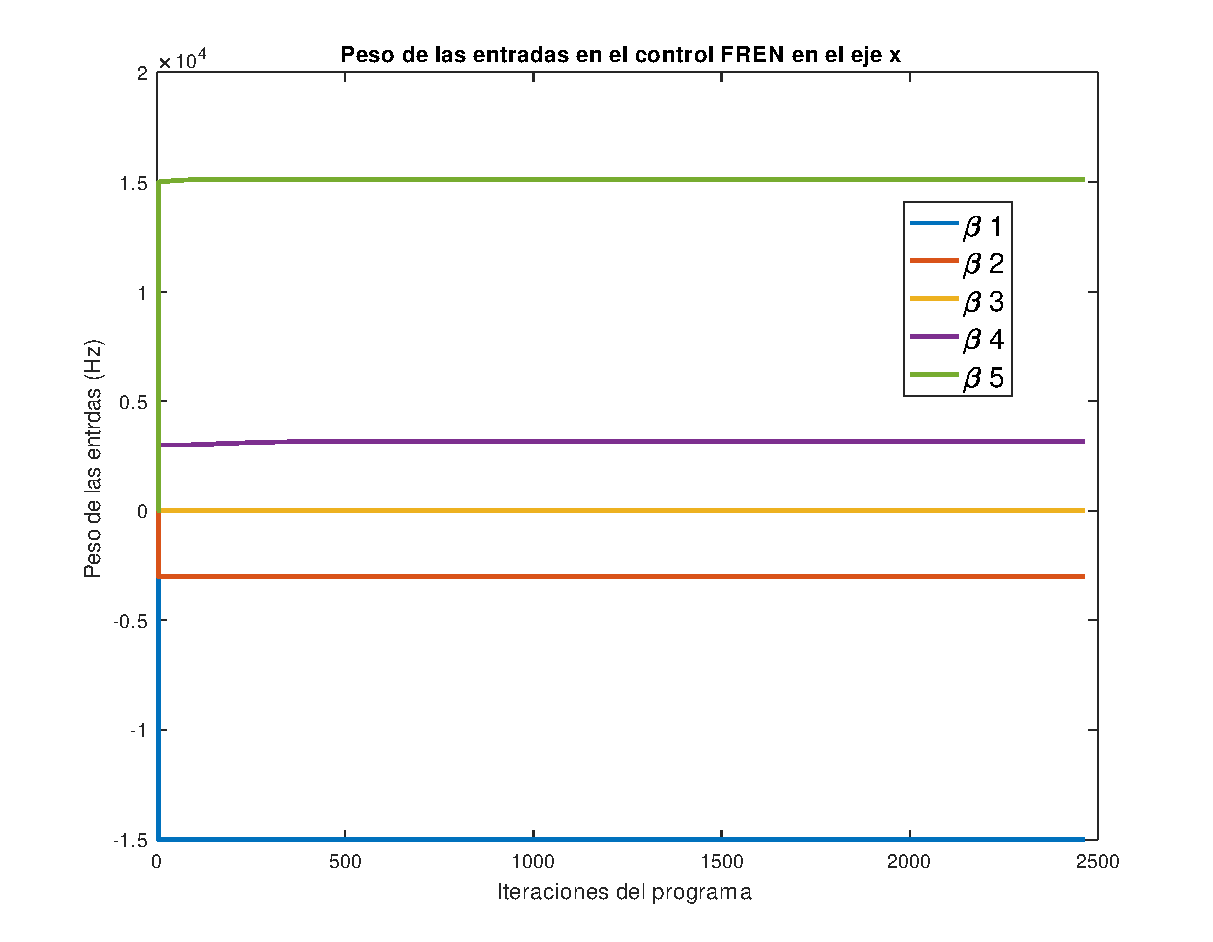
\includegraphics[width=1\linewidth]{visio/graficasderesultados/betasx1}
	\caption{Valores de $\beta$ del eje x}
	\label{fig:betasx1}
\end{figure}
\begin{figure}
	\centering
	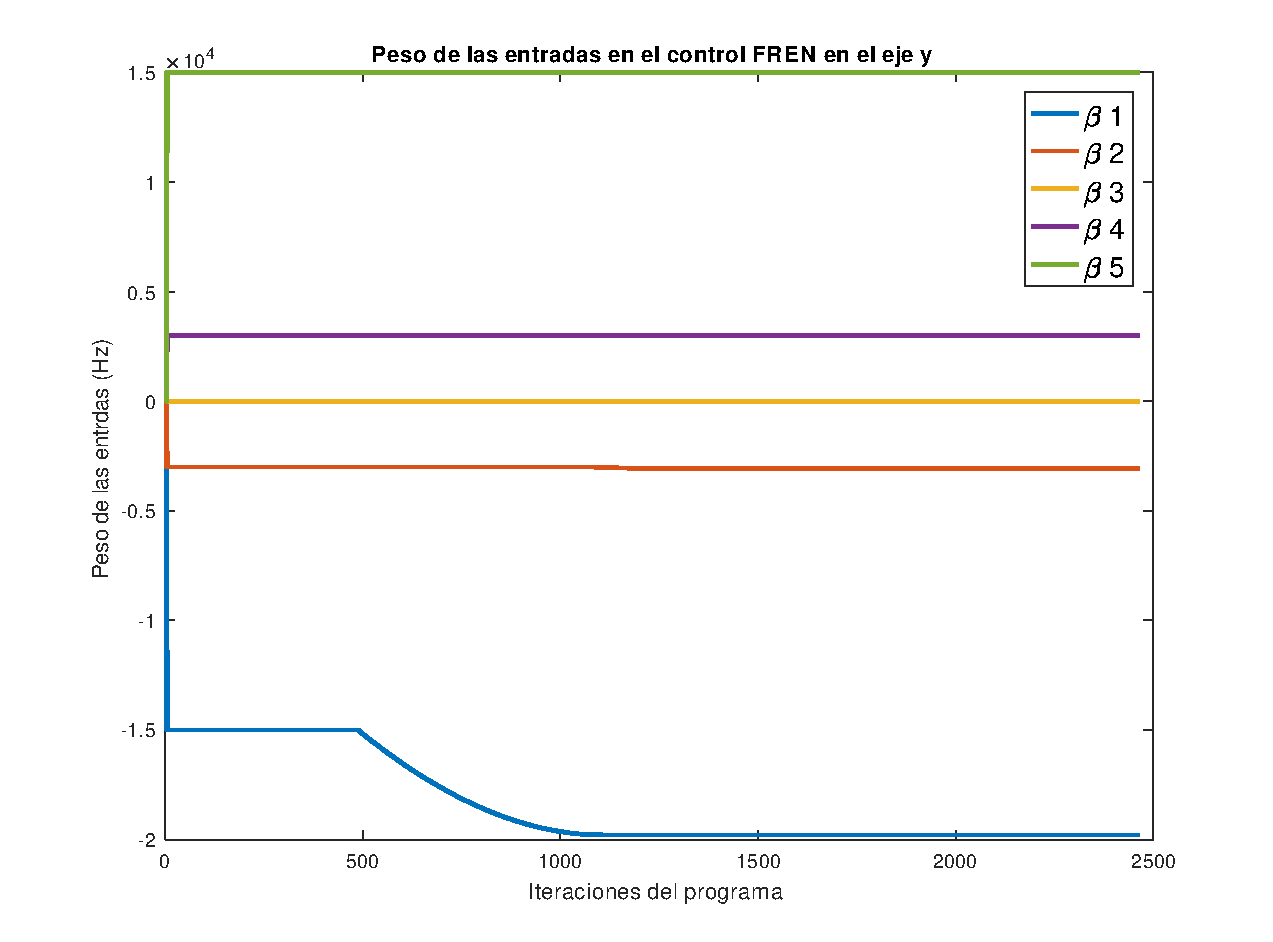
\includegraphics[width=1\linewidth]{visio/graficasderesultados/betasy1}
	\caption{Valores de $\beta$ del eje y}
	\label{fig:betasy1}
\end{figure}
\begin{figure}
	\centering
	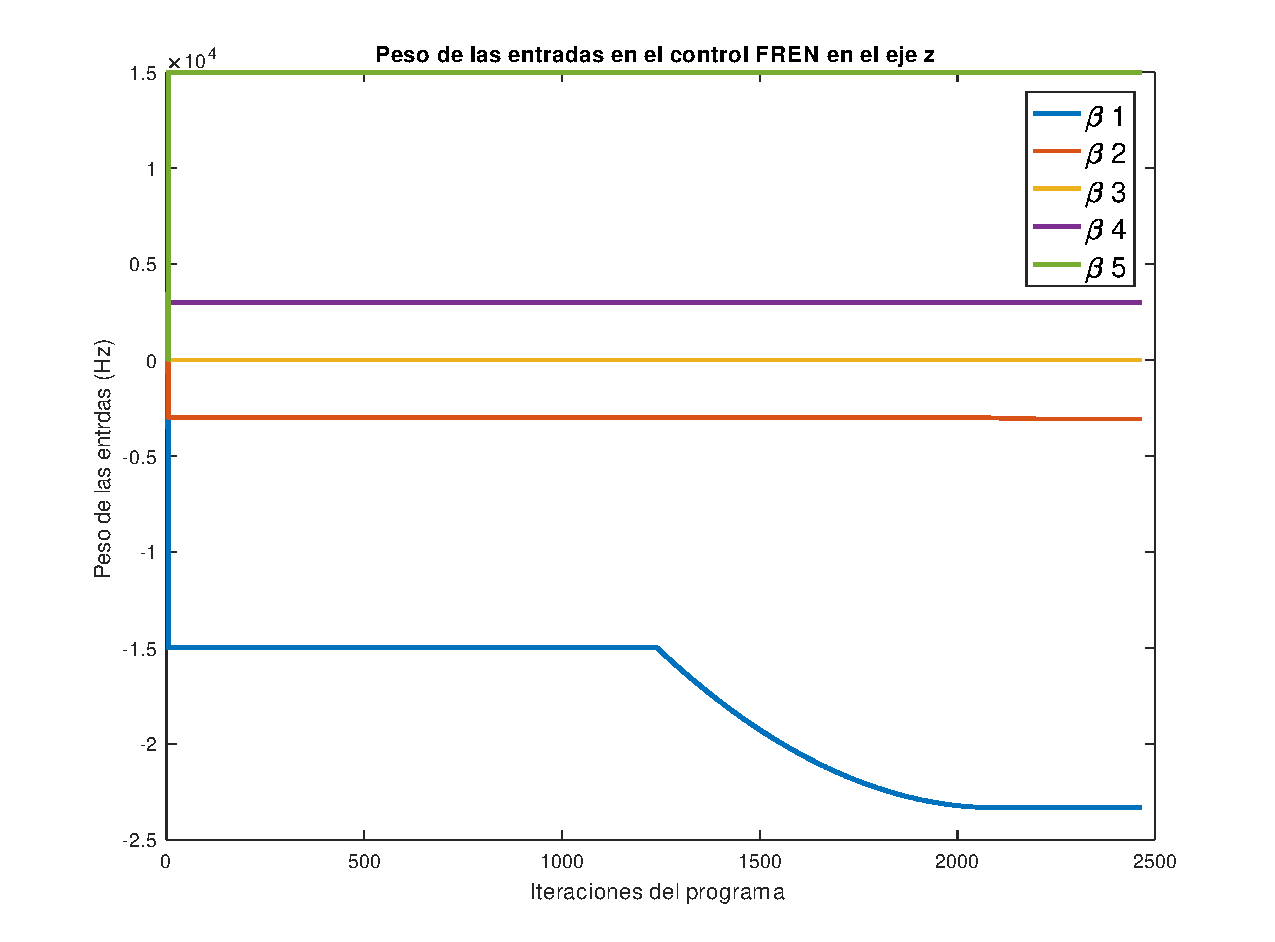
\includegraphics[width=1\linewidth]{visio/graficasderesultados/betasz1}
	\caption{Valores de $\beta$ del eje z}
	\label{fig:betasz1}
\end{figure}
\begin{figure}
	\centering
	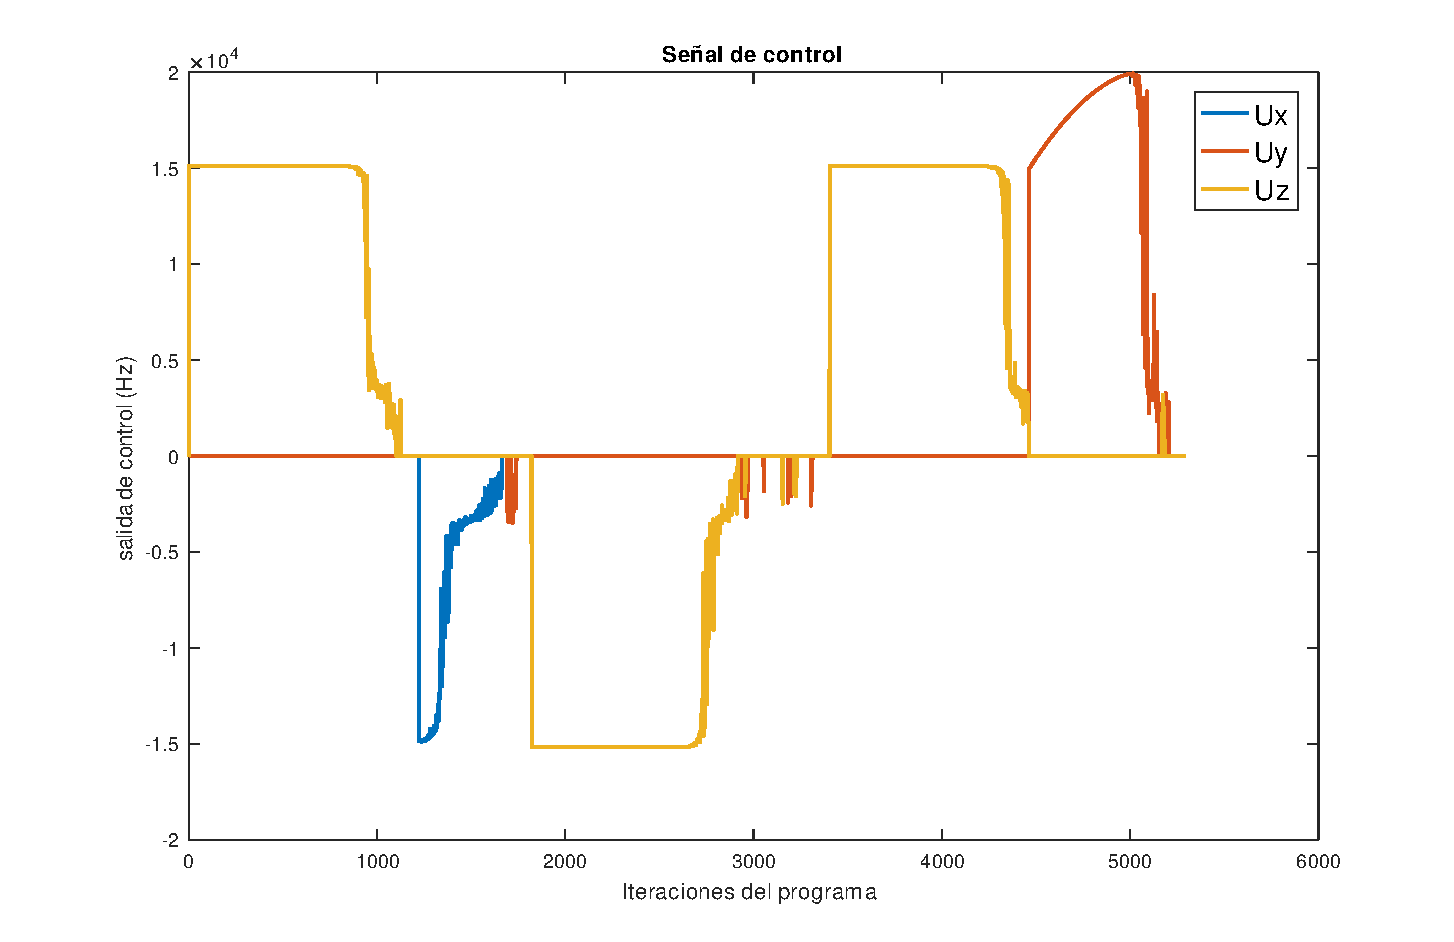
\includegraphics[width=1\linewidth]{visio/graficasderesultados/control1}
	\caption{}
	\label{fig:control1}
\end{figure}

\begin{figure}
	\centering
	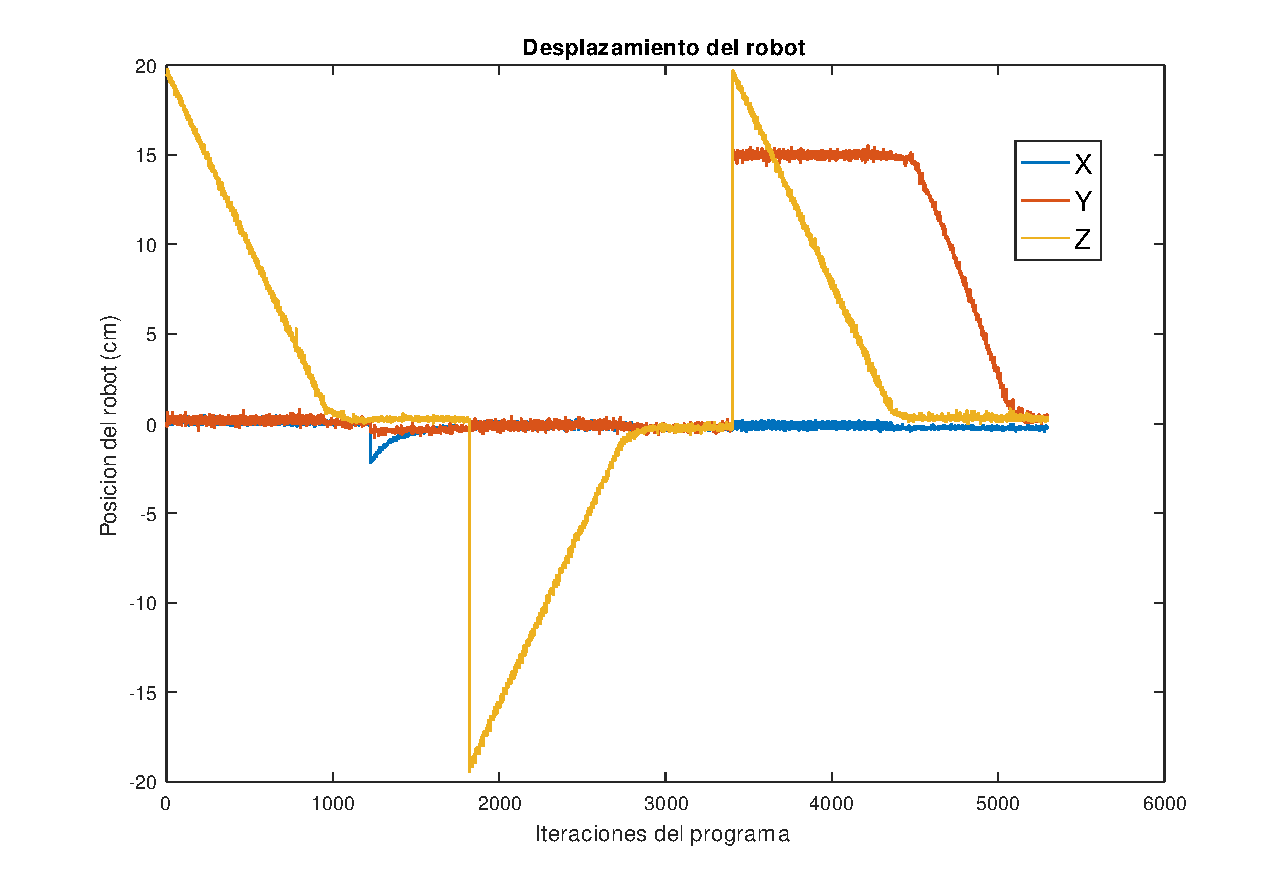
\includegraphics[width=1\linewidth]{visio/graficasderesultados/posicion1}
	\caption{}
	\label{fig:posicion1}
\end{figure}




en \cref{tab:result1}se muestran los resultados de distintos experimentos, aquí se muestra que existe los estos son repetibles.
en cada uno de los experimentos, el objeto fue colocado en un lugar aleatorio.
No se realizaron experimentos con ningún objeto que no pudiera ser detectable, o no pudiera ser levantado.
\\



\begin{table}[h]
	\caption{Estadisticas de los experimentos realizados} \label{tab:result1} 
	\centering
	\footnotesize 
\begin{tabular}{|c||c|c|c|c|c|}
\hline
objetos	 & numero de experimentos & experimentos exitosos  & notas\\
\hline  
\hline  
baso & 10  & 10 &  baso de unicel   \\
pelota & 10 &  10 &  pelota de plastico  \\
manzana & 10 &  10 & manzana verde \\ 
caja de carton & 10 &  10 & caja de carton  \\
% & ???? &  ???? &  ??? \\
\hline 
\end{tabular} 
	\bigskip
\\
\end{table}

\clearpage



Los resultados del sensor de fuerza y momentos se pueden ver en  \cref{fig:twist1}, la gráfica representa las fuerzas a lo largo de todo el experimento, desde el momento en el que se toma la primer imagen hasta el momento en que se llega a la posición final y termina. en general se puede observar fácilmente como al principio esta en calma, pero después de comienza a haber una gran cantidad de ruido, este ruido  se debe por las vibraciones de uno de los ejes de robot, en el momento en que se cierra es cuando aumentan abrupta mente los valores, y toma un instante en conseguir estabilizar los valores, después se puede encontrar m,as ruido, el cual de nuevo es debido a las vibraciones producidas por el robot.
una vez se libera el objeto en el punto designado, el \textit{Gripper} se mueve hasta un área de \textit{Home}, pero en el trascurso de esto se puede notar mas ruido.

Vale la pena analizar un poco mas a fondo esta respuesta, ya que en \cite{keylist}, se habla de como las vibraciones en los sensores piezoelectricos 
Aun cuando es considerable la diferencia entre este sensor y los piezoelectricos, esta claro en \cref{fig:pelota1}, que al ocurrir deslizamiento, se general vibraciones.
A continuación se muestran los espectrogramas de cada una de las señales de \cref{fig:twist1}, en estas se puede observar 2 características principales, la primera es que existen frecuencias altas en el instante en que se realiza la sujeción, esto es simplemente debido al cambio repentino, y la segunda característica es las bajas frecuencias que se presentan en el resto del experimentos, esto ori haber sido, porque las frecuencias del deslize del objeto son demaciado bajas, pero tambin podria significar que las frecuencias bajas son debidas a las vibraciones del robot y estas al ser mecanincas son de baja frecuencia.










\begin{figure}
	\centering
	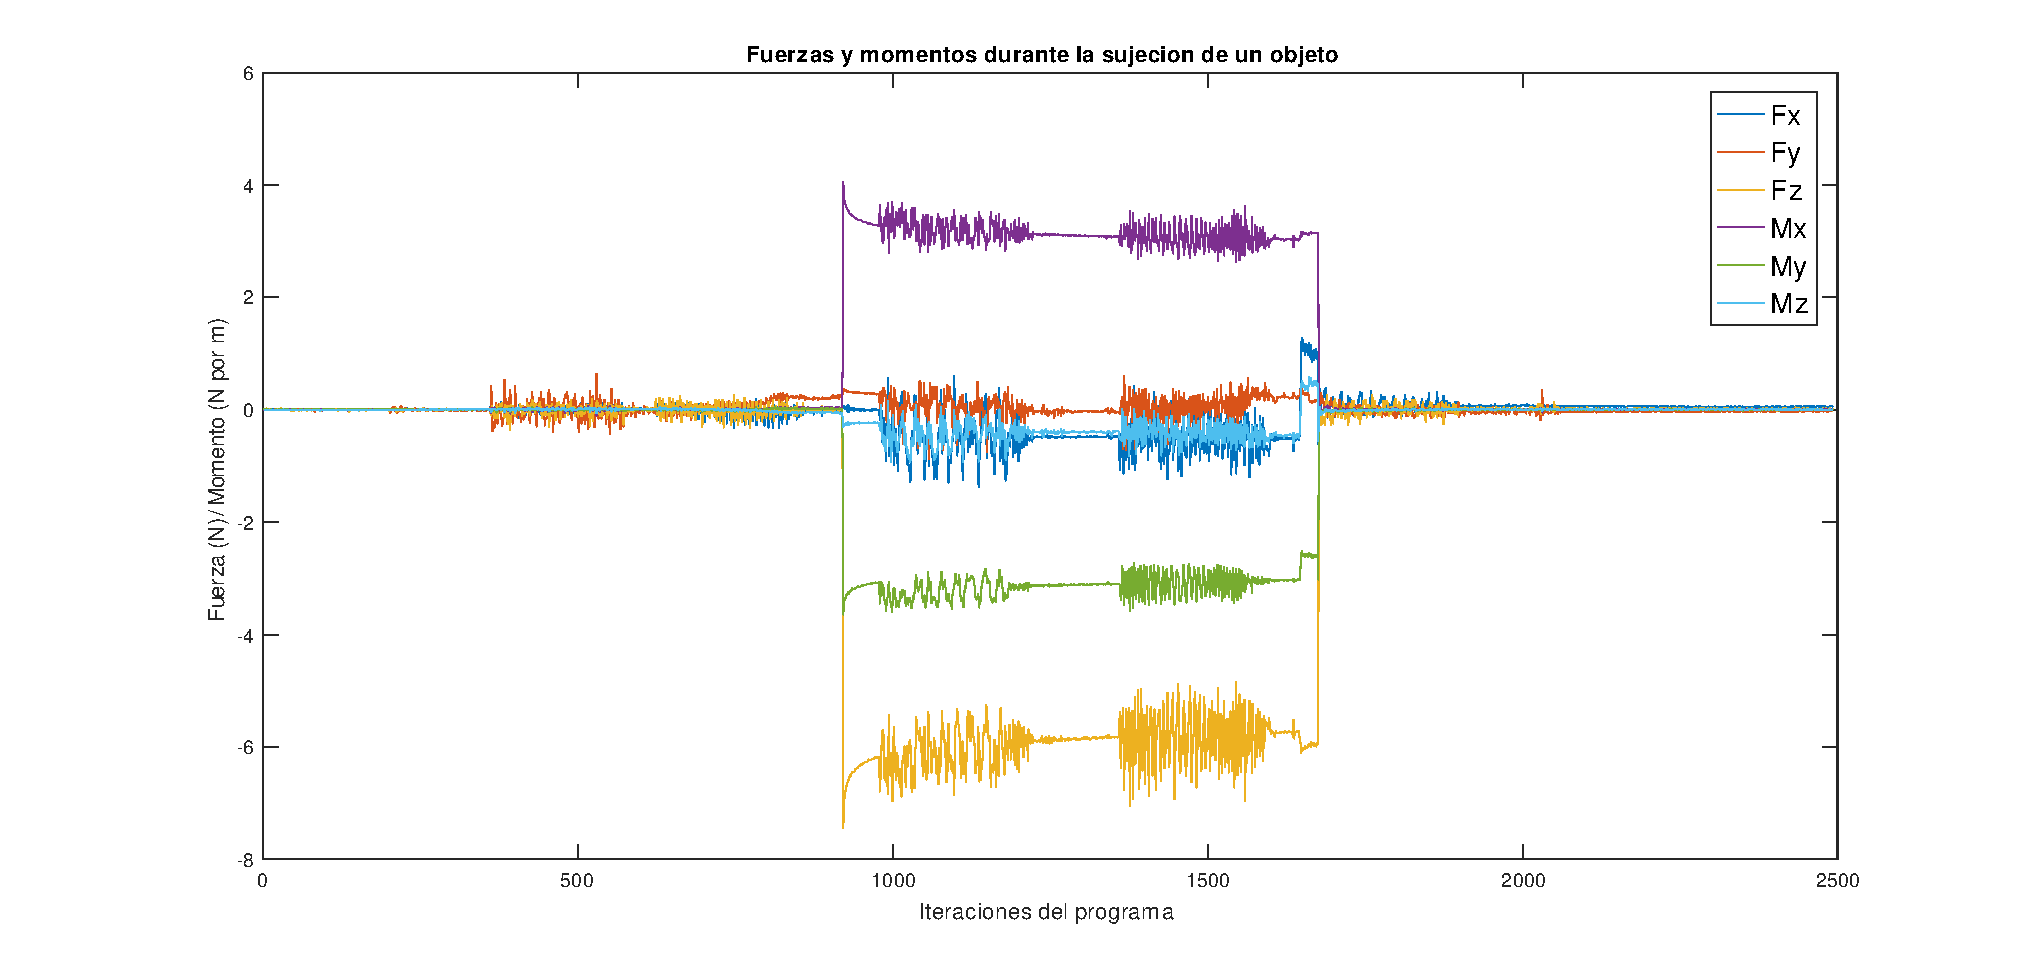
\includegraphics[width=1\linewidth]{visio/graficasderesultados/twist1}
	\caption{Fuerzas y momentos mecánicos involucrados en el agarre}
	\label{fig:twist1}
\end{figure}


\begin{figure*}[h]
	\centering
	\begin{tabular}{cccc}
		%\hline 
		\subfloat[Objeto Segmentado]{		\includegraphics[width=.48\linewidth]{visio/graficasderesultados/pelota11}\hspace{1cm}\label{Fx}}
		
		\subfloat[sobel en x]{%
			\includegraphics[width=.48\linewidth]{visio/graficasderesultados/pelota12}\label{Fy}}
		\\
		\subfloat[sobel en y]{%
			\includegraphics[width=.48\linewidth]{visio/graficasderesultados/pelota13}\hspace{1cm}\label{Fz}}
		\subfloat[sobel en y]{%
			\includegraphics[width=.48\linewidth]{visio/graficasderesultados/pelota14}\label{Mx}}
			\\
		\subfloat[sobel en y]{%
			\includegraphics[width=.48\linewidth]{visio/graficasderesultados/pelota15}\hspace{1cm}\label{My}}
		\subfloat[sobel en y]{%
			\includegraphics[width=.48\linewidth]{visio/graficasderesultados/pelota16}\label{Mz}}
		%	\hline 
	\end{tabular}
	\caption{Espectrogramas de los valores del sensor}
	\label{fig3} 
\end{figure*}
\clearpage
Para observar las frecuencias que ocurrirían comúnmente en el desliz de un objeto, se realizó una serie de  experimentos en los que simplemente se tuviera un objeto sujetado en el \textit{Gripper}, y fuera deslizado manualmente, esto para evitar las vibraciones del robot, aunque se tendrían las irregularidades de un ser humano, pero se esperaba que estas fueran irregulares y lentas y no afectaran las verdaderas vibraciones del desliz.

A continuación se muestran los resultados de experimentos que se hicieron específicamente para observar el deslizamiento de una pieza.

en el experimento se comienza por sujetar el objeto y después de un tiempo se deja que la señal se estabilice, una vez sucede esto se comienza a jalar el objeto hasta que termina de salir.Este experimento en especifico se realizo con una pelota de plástico.

Lo que se puede observar al principio de \cref{fig:pelota1} e que no tiene la cantidad de ruido que se tenia en \cref{fig:twist1}, lo cual no ayudara a tener resultados mas claros, lo importante es que aun cuando se ha sujetado e objeto se continua sin tener ruido considerable, pero cuando se comienza a deslizar el objeto, se puede observar las vibraciones en la señal, lo cual indica que realmente están ahí cuando el objeto se desliza. por ultimo y mas importante es el hecho de que la señal $M_y$, comienza a mover sus valores dependiendo de cuanto s ha deslizado el objeto,  esta es na de las características que se esperaban, ya que esta es un indicador de la posición del objeto, y su razón de cambio indica que tanto se esta deslizando el objeto, pero no se toma n cuenta del todo por que es una propiedad que depende de la geometría del objeto, por lo que no siempre se comportara de la misma manera, por ejemplo se puede observar en \cref{fig:pelota1}, como después de un tiempo comienza a subir la señal. Aun después de ese inconveniente, no se puede ignorar que es un buen indicador del desliz.

ahora, la razón por la que se prefiere usar las vibraciones de las señales como indicador, incluso si esta señal ya nos proporciona información, es porque las vibraciones nos podrían indicar el desliz en todo momento, aunque el desliz sea mas lento o mas rápido, sin importar la geometría del objeto, simplemente se usaría un filtro pasa-banda para encontrar las frecuencias deseadas  ignorar el resto, por esta razón se analizaron mas a fondo estas señales.
en  la \cref{fig:pelota1x} hasta \ref{fig:pelota1c}, se encuentran los espectrogramas de \cref{fig:pelota1}, en estas figuras, por desgracia no se encuentra la información necesaria por el hecho de que las frecuencias eran demasiado bajas, y muy tenues.
\begin{figure}
	\centering
	\includegraphics[width=1\linewidth]{visio/graficasderesultados/pelota1}
	\caption{}
	\label{fig:pelota1}
\end{figure}
\begin{figure}
	\centering
	\includegraphics[width=0.7\linewidth]{visio/graficasderesultados/pelota1a}
	\caption{}
	\label{fig:pelota1a}
\end{figure}
\begin{figure}
	\centering
	\includegraphics[width=0.7\linewidth]{visio/graficasderesultados/pelota1b}
	\caption{}
	\label{fig:pelota1b}
\end{figure}
\begin{figure}
	\centering
	\includegraphics[width=0.7\linewidth]{visio/graficasderesultados/pelota1c}
	\caption{}
	\label{fig:pelota1c}
\end{figure}
\begin{figure}
	\centering
	\includegraphics[width=0.7\linewidth]{visio/graficasderesultados/pelota1x}
	\caption{}
	\label{fig:pelota1x}
\end{figure}
\begin{figure}
	\centering
	\includegraphics[width=0.7\linewidth]{visio/graficasderesultados/pelota1y}
	\caption{}
	\label{fig:pelota1y}
\end{figure}
\begin{figure}
	\centering
	\includegraphics[width=0.7\linewidth]{visio/graficasderesultados/pelota1z}
	\caption{}
	\label{fig:pelota1z}
\end{figure}


\clearpage
\section{Conclusiones}

Uno  de los mayores inconvenientes fue el \textit{Gripper}, el tiempo de respuesta del \textit{Gripper} no es tan bueno como se esperaría, esto debido a las capas de comunicación que existen, estas impiden que las instrucciones sean ejecutadas rápidamente, esto por lo general no representa un problema demasiado grande, pero en aplicaciones donde es necesario cancelar una de las instrucciones que se están llevando a cabo, para realizar otra que tenga mayor prioridad, el problema de las herramientas de arquitectura cerrada, por lo que se resolvería sise cambiara a uno  de arquitectura abierta, este ultimo recibiría entradas de control directamente, en lugar de instrucciones, por lo que seria mas flexible.


Los resultados de los algoritmos fueron lo suficiente mente buenos como para lograr el agarre del objeto en cada experimento con un cierto objeto.
Es un hecho que existe error en la señal de la imagen de entrada, en el procedimiento que se lleva a cabo para encontrar el centroide del objeto (mas importante aun en el hecho de usar el centroide como punto de agarre), y finalmente en el posicionamiento, en el cual se desactiva el control cuando se esta a medio centímetro de la posición indicada, pero pese a esto, se logro llegar y sujetar los objetos que se tenían como objetivo.

Se presento una tabla con resultados que mostraban como era posible conseguir el agarre en varios experimentos, mostrando que es repetible, pero la tabla solo mostraba los experimentos que se habían realizado con una pequeña cantidad de objetos, en caso de existir mas de un objeto en escena lo que se hace es tomar el que esta mas cercano a la cámara, pero aun así, existieron una serie de experimentos que no pudieron ser presentados, estos son aquellos en que no se pudo conseguir una  imagen aceptable del objeto por el hecho de reflejar demasiado la luz, en cuyo caso es inútil intentar mas con el equipo que se tiene, otra situación parecida es cuando el objeto era demasiado pequeño para poder ser detectado de forma correcta, el objeto mas pequeño que se detecto fue un lápiz.

Los casos mas importantes fueron los experimentos en los que se tenia un objeto con forma irregular que tuviera el centroide fuera del cuerpo. existían casos en que aun siendo un objeto irregular, pero el centroide se encontraba dentro del cuerpo, entonces el objeto podía ser sujetado sin, pero esto también nos lleva a otro caso, en el que el punto que se usaba para sujetar no es el adecuado, un ejemplo de esto es un objeto que no tenga un punto de agarre adecuando en el centroide. Estos casos no pueden ser solucionados por culpa del algoritmo usado, , 



El ultimo caso de experimentos fallidos, es los casos en los que el objeto pesaba mas de lo que se esperaba, por lo general este no seria un problema si no fuera por el hecho de que el \textit{Gripper} no es capaz de responder suficientemente rápido a las ordenes. Por ejemplo, en \cref{fig:pelota1}, se muestra como, en la linea verde, la cual representa el momento mecánico en el eje Y, es un muy buen indicador para el deslizamiento, pero por desgracia, durante los experimentos, el \textit{Gripper}, no respondió de la manera esperada y en varias ocasiones se dieron fallos de comunicación, por intentar detener el comando actual y cambiar los parámetros, o simplemente se dieron casos en los que se tardaba tanto que no pudo ser utilizable, ya que la velocidad de respuesta es de 1 segundo cuando no se encuentra ocupado y de 2 a 3 segundos cuando se encuentra ocupado, la situación de esos 3 segundos es cuando se encuentra en sujeción, aun cuando existe un paro de emergencia, esto solo detendría la ejecución de la orden actual, pero no permitiría comenzar una nueva, ya que el \textit{Gipper}, no puede ser usado hasta que se remueva ese estado de \textbf{Error}, y en algunos casos se puede dar un  error por tiempo.


